\documentclass{beamer}
\usetheme{Madrid}
\setbeamertemplate{itemize item}[triangle]
\usecolortheme{whale}
\beamertemplatenavigationsymbolsempty

\usepackage{fontspec}
% \usepackage[czech]{babel}
\usepackage{siunitx}
\sisetup{
	list-units           = single,
	list-separator       = {; },
	range-units          = single,
	detect-all,                            % Use sans-serif
}
\DeclareSIUnit\arbunit{rel.~j.}

\usepackage{graphicx}
\graphicspath{
	{../img/}
	{img/}
}
\usepackage[outdir=build/plots/]{epstopdf}
\usepackage{tikz}

\usetikzlibrary{arrows.meta}
\usetikzlibrary{bending}
\usetikzlibrary{positioning}

\tikzset{
	level/.style = {},
	transition/.style = {
		thick,
		arrows = {-Latex},
	}
}

\DeclareSIUnit\sccm{sccm}
\DeclareSIUnit\arbunit{rel.\ j.}

\newcommand\eu{e}
\newcommand\im{i}

\newcommand\lightspeed{c}
\newcommand\planck{h}

\newcommand\efishsetup{
}

\newcommand\kryptontalifgrotrian{
	\draw [level] (4,0) -- (6,0)
		node [right] {$\mathrm{4p^6\ {}^1S_0}$};
	\draw [level] (4,10) -- (6,10)
		node [right] {$\mathrm{5p'\ [3/2]_2}$};
	\draw [level] (3,6) -- (1,6)
		node [left] {$\mathrm{5s'\ [1/2]_1}$};

	\draw [transition] (5,0) -- (5,5);
	\draw [transition] (5,5) -- (5,10);
	\path (5,0)
		-- node [sloped, below] {$2 \times \SI{204.13}{\nano\metre}$} (5,10);
	\draw [transition] (5,10)
		-- node [sloped, above] {$\SI{826.3}{\nano\metre}$} (2,6);
}

\newcommand\lifgrotrian{
	\draw [level] (4,0) -- (6,0)
		node [right] {$1$};
	\draw [level] (4,10) -- (6,10)
		node [right] {$3$};
	\draw [level] (3,6) -- (1,6)
		node [left] {$2$};

	\draw [transition] (5,0) -- (5,10);
	\path (5,0)
		-- node [sloped, below] {laserová excitace} (5,10);
	\draw [transition] (5,10)
		-- node [sloped, above] {LIF} (2,6);
}

\newcommand\seleniumlifgrotrian{
	\draw [level] (4,0) -- (6,0)
		(5,-1) node {$4s^2 4p^4\ {}^3\mathsf{P}_2$};
	\draw [level] (4,10) -- (6,10)
		(5,11) node {$4s^2 4p^3({}^4\mathsf{S}^o) 5s\ {}^3\mathsf{S^o}_1$};
	\draw [level] (3,6) -- (1,6)
		node [left] {$4s^2 4p^4\ {}^1\mathsf{S}_0$};

	\draw [transition] (5,0) -- (5,10);
	\path (5,0)
		-- node [sloped, below] {\SI{196.09}{\nano\metre}} (5,10);
	\draw [transition] (5,10)
		-- node [sloped, above] {\SI{350.25}{\nano\metre}} (2,6);
}


\title[Laser plasma diagnostics]
{Plasma diagnostics by means of a picosecond laser}
\subtitle{Diploma thesis}
\date{2023}
\author{Jan Slaný}
\institute[PřF MUNI]{Faculty of Science, Masaryk University\\
	Department of Physical Electronics}

\newcommand\elfield{E}
\newcommand\efish{I_{2\omega}}
\newcommand\tim{t}

\begin{document}

\begin{frame}[plain]
	\titlepage
	\footnotesize
	Supervisor: doc. Mgr. Pavel Dvořák, PhD.
\end{frame}

\begin{frame}
	\frametitle{EKSPLA Picosecond Laser}
	\begin{columns}
	\begin{column}{0.5\textwidth}
		\begin{itemize}
			\item Nd:YAG ($\SI{1064}{\nano\metre}$)
			\item adjustable wavelength
			\item pulse duration $\SI{30}{\pico\second}$
			\item pulse energy $\SI{30}{\milli\joule}$
		\end{itemize}
	\end{column}
	\begin{column}{0.5\textwidth}
		\begin{figure}
			\centering
			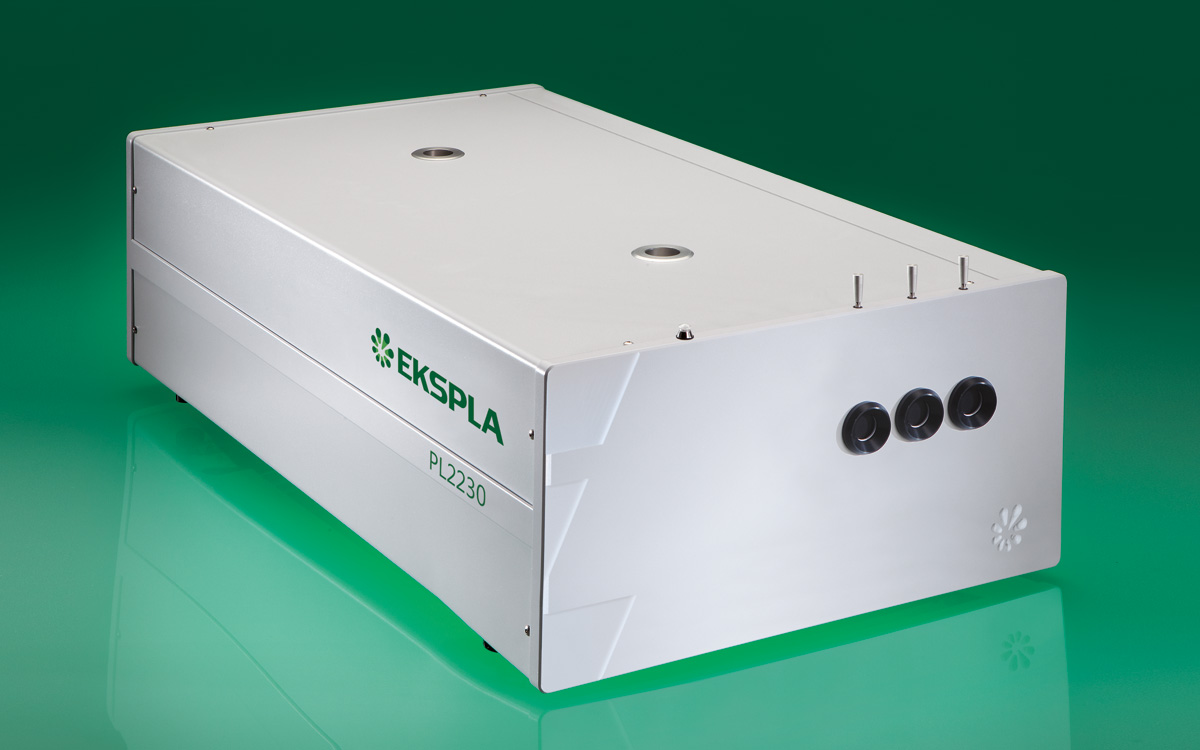
\includegraphics[width=\textwidth]{laser}
			\caption{The \emph{EKSPLA PL2231-50} laser.
				From \texttt{ekspla.com}.}
		\end{figure}
	\end{column}
	\end{columns}
\end{frame}

\section[E-FISH]{Electric field induced second harmonic generation}

\begin{frame}
	\frametitle{E-FISH}
	\begin{itemize}
		\item non-linear optical environment or high intensity
		\item two photons of equal frequency combine to form
			a new one with double frequency
		\item $\efish \sim (I_\mathrm{laser} \elfield)^2$
	\end{itemize}
\end{frame}

\begin{frame}
	\frametitle{Discharge}
	\begin{columns}[c]
	\begin{column}{0.5\textwidth}
		\begin{itemize}
			\item atmospheric pressure dielectric barrier discharge
				in $\mathrm{N}_2$
			\item 2\times microscope slide \SI{1.1}{\milli\metre}
			\item \SI{1}{\milli\metre} gap
			\item \SI{11}{\kilo\hertz}, \SI{14}{\kilo\volt}
		\end{itemize}
	\end{column}
	\end{columns}
\end{frame}

\begin{frame}
	\frametitle{Calibration}
	\sisetup{per-mode=symbol}
	\graphicspath{{../efish/}}
	\input{../efish/plots/calib}
\end{frame}

\begin{frame}
	\frametitle{Electric field in discharge}
	\begin{figure}
		\centering
		\small
		\sisetup{per-mode=symbol}
		\graphicspath{{../efish/}}
		\input{../efish/plots/period-elfield}
		\caption{Spatial and temporal evolution of the intensity
			of electric field in the discharge over one period.}
	\end{figure}
\end{frame}

\section[TALIF]{Two-photon absorption laser-induced fluorescence}

\section{Summary}
\begin{frame}
	\frametitle{Summary}
	Done:
	\begin{itemize}
		\item apply E-FISH to electric field determination
		\item TALIF, LIF preliminary results
		\item discovered variation in the laser beam profile
			(partial correction using a spatial filter)
	\end{itemize}
	\bigskip
	To do:
	\begin{itemize}
		\item redo TALIF
		\item Raman\dots
	\end{itemize}
\end{frame}

\end{document}
